\chapter{Essential Economics}
This chapter discusses terminology, stock market dynamics, and important indicators in economics. This will allow us to more accurately judge the value of an economic decision and make predictions on the market.

\section{Funds}

We'll discuss three different types of funds: \acf*{etf}, mutual funds, and hedge funds. Different types of funds are governed under different rules. \ac*{etf}s are similar to stocks in that they are bought and sold at will like stocks- very liquid. However, \ac*{etf}s typically represent baskets of stocks, and it is known to the trader what the fund represents. Mutual funds can only be bought and sold at the end of the day, and the holdings within a mutual fund are only disclosed every quarter. The least transparent holdings are that of a hedge fund. Before investors can buy shares in the fund, they must sign a long term agreement and holdings are rarely disclosed. \\

\subsection{About Funds}

For stocks and \ac*{etf}s, having a large "cap" means that the total value of stocks (number of stocks $\times$ price of a stock) in a company is worth many billions of dollars. Moreover, the price of a stock doesn't reflect the value of a company, but the price at which they are selling shares. \ac*{etf}s, like stocks, can easily be traded through individuals alone, whereas shares in mutual funds require a broker and hedge fund shares require more of a one on one relationship. Managers of \ac{etf}s and mutual funds are compensated based on expense ratios, which denote a percentage of \ac{aum}. For an \ac{etf}, expense ratios range from 0.01\% to 1\%, and in mutual funds from 0.5\% to 3\%. Hedge funds follow a "two and twenty" policy, where managers get 2\% of the \ac{aum} and 20\% of the profits.\\

The type of a fund can be more easily recognized by how it's named. For example, an \ac*{etf} has a ticker, or stock symbol, with three or four letters, like AAPL. A mutual fund has five letters, like VTINX, and a hedge fund doesn't have a ticker because shares are much less liquid. How much money is managed by a fund is known as the \ac{aum}, and shares represent percentages of the \ac{aum}. \\

It's fairly clear to see that hedge funds are very different from \ac{etf}s and mutual funds. Hedge funds typically have no more than 100 investors, whereas \ac{etf}s and mutual funds have thousands. Those that invest in hedge funds are typically very wealthy individuals, institutions, and funds of funds. Funds of funds typically take large sums of money from potentially many places and invest in several hedge funds. This is a bridge for smaller investors to participate in hedge fund. The goal of a hedge fund typically falls along the lines of two ideals. The hedge fund may be out to beat a bench mark which is to say that the hedge fund aims to outperform an index of stocks. A hedge fund could also aim for absolute return, which translates to net positive profit no matter what, but usually takes more time and has fewer returns as a trade off for stability. We'll be focusing on hedge funds because they are the most computationally demanding.

\subsection{Fund Metrics and Operations}
Measuring the performance of a fund is vital for making financial decisions in the market, so here we'll discuss a few. Overall success can be measured by cumulative return, which is the percentage of an original value made in a given time: $\frac{end-start}{start}$. However, this means little if the portfolio is rapidly and wildly fluctuating. Hence it's also useful to measure the volatility of a portfolio. This is simply measured by the standard deviation of daily returns; it's best to have low volatility. Another important measure is the return on risks. This is done by calculating the \ac{sr}, also called risk-adjusted reward. 
\begin{align*}
\ac{sr}=\frac{mean(\mbox{daily returns}-\mbox{risk free rate})}{\mbox{volatility}}\sqrt{252}
\end{align*}
The factor of $\sqrt{252}$ comes from the number of trading days in a year. These factors can give us an idea of how well a portfolio is performing.\\

As previously mentioned, hedge funds are very computationally intensive environments. Let's delve into the details of how a typical hedge fund works. Central to the operation of a hedge fund is its trading algorithms. Normally, a target portfolio is decided upon, then historical stock data and the target portfolio are fed to the trading algorithms to produce orders. The orders are sent to the market to alter the live portfolio, which is again fed back into trading algorithms. 
\newpage

\begin{figure}[h!]
\begin{center}
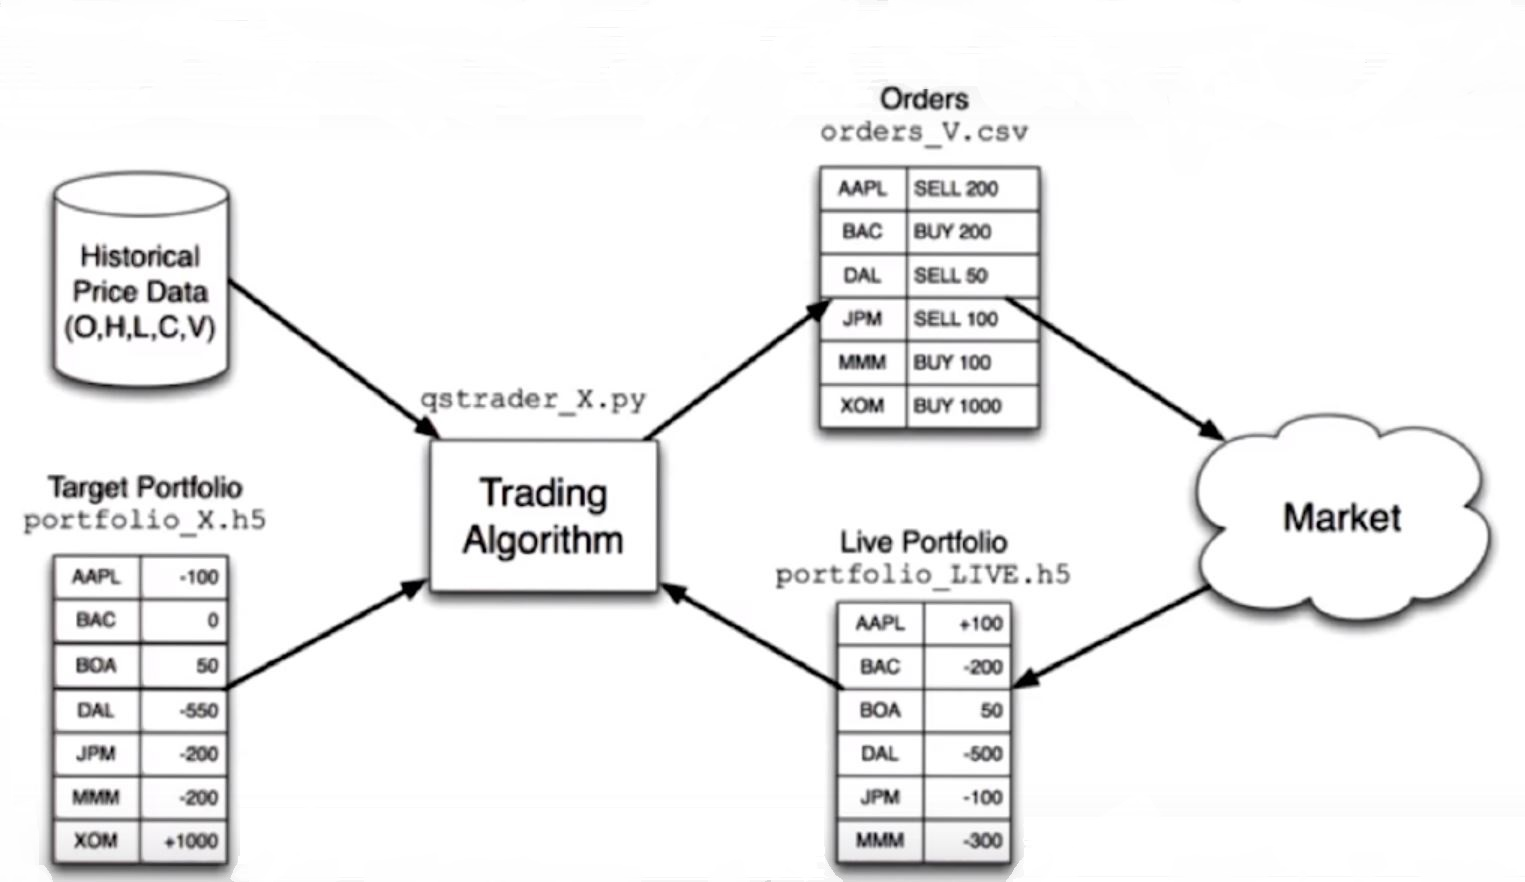
\includegraphics[scale=.4]{images/operation.JPG}
\caption{Graphical representation of hedge fund operation.}
\end{center}
\end{figure}

Trading algorithms work to place certain orders at the proper time. For example, an order for everything in the target portfolio shouldn't be placed all at once because the price of the stock will go up and more money is spent than if strategic ordering were implemented. Additionally, there is another set of computational structures for determining the target portfolio.

\begin{figure}[h!]
\begin{center}
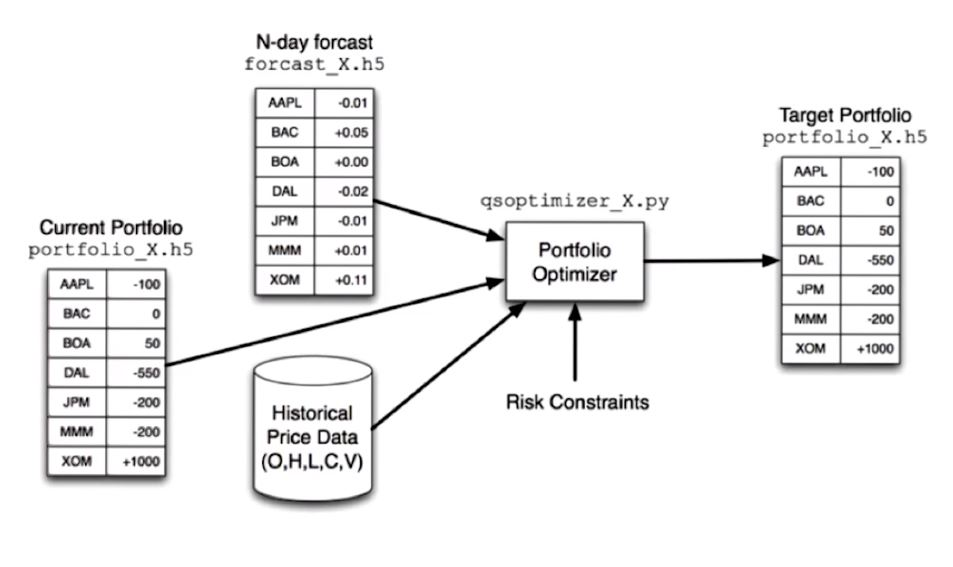
\includegraphics[scale=.75]{images/target.JPG}
\caption{Producing a target portfolio.}
\end{center}
\end{figure}

Historical data, current portfolio, and prediction algorithms are fed into an optimization program to produce a target portfolio. The majority of machine learning comes into play when determining the market forecast. 

\section{Market Mechanics}

\subsection{Ordering}
The live portfolio is altered by giving orders to a broker in the stock market, so it serves to know what exactly is in an order. The broker needs to know whether to buy or sell and of which stock(s) by their market symbols. The order must also contain the number of shares and the type of order. Stock exchanges only consider limit orders and market orders, but note that orders can be increasingly complex based on instructions given to a broker. A market order is an order at the current market price, and ordering at a limit price tells the broker to only buy or sell at a certain price; for example, some may not want to buy beyond some value or sell below some price. Of course, a limit order must also include the desired price. \\

\begin{table}[h!]
\centering
\begin{tabular}{c|c|c|c|c}
BUY/SELL & SYMBOL & SHARES & TYPE & PRICE \\
\hline
BUY & IBM & 100 & MARKET & - \\
BUY & AAPL & 500 & LIMIT & 100 \\
SELL & FB & 1000 & LIMIT & 110 \\
BUY & GOOG & 100 & LIMIT & 740 \\
SELL & NFLX & 50 & MARKET & - \\
SELL & GE & 50 & LIMIT & 40 \\
\end{tabular}
\caption{Example list of orders.}
\end{table}

After the broker sends the order to the stock exchange, it is made public in the style of an "order book". Others can see the stocks and collective bids that have been made on them, but not who has placed the orders. The order book contains a list for each stock of the orders within it including whether the order asks for others to buy or bids on the stock. Both types include a price at which orders are allowed to be bought/sold at and the size of the order. Orders of the same type and price are lumped together. Market orders always sell at the highest bid and buy at the lowest asking price. \\

\begin{table}[h]
\centering
\noindent\begin{tabular}{c@{}l}
  \begin{tabular}{c|c|c}
  	BID/ASK & PRICE & SIZE \\
    \hline
    ASK & 100.10 & 100 \\
	ASK & 100.05 & 500 \\
	ASK & 100.00 & 1000 \\
	BID & 99.95 & 100 \\
	BID & 99.90 & 50 \\
	BID & 99.85 & 50 \\
  \end{tabular} 
  & 
  $\begin{array}{l}
  \\
    \MyLBrace{5ex}{SELL} \\ 
    \MyLBrace{5ex}{BUY} \\ 
  \end{array}$
\end{tabular}
\caption{Example order book.}
\end{table}

The example order book suggests that the price of the stock will decrease because there is much more selling pressure- more are selling than buying. \\

\subsection{Dynamics of Exchange}
There are many stock exchanges, and each has its own order book. When an order is placed, say by an individual, the order is sent to the broker and the broker chooses between the stock exchanges to execute that order. The broker takes information from all the stock exchanges and makes a transaction based on which one has the stock with the best price. Fees are associated with making transactions in stock exchanges and with using a broker. A broker typically has many clients; the broker can observe clients who want to buy and sell at the same price and circumvent stock exchanges entirely. The law ensures that this trade can only happen if both the buyer and seller get prices that are at least as good as at an exchange. Even if this transaction cuts out the stock exchange, it must still be registered with one, and it's usually with the exchange the stock is housed. \\

Orders can be handled internally or moved through what's called a "dark pool". A dark pool is a place where investors can trade without the transparency of an order book outside of a stock exchange. The results of the trade, like internal trades, still need to be registered with public exchanges after they've occured. A dark pool can act as an intermediary between all types of investors that may want to escape the transparency of stock exchanges. Brokers like this because they don't have to pay fees associated with trading at a stock exchange. They also argue that it's fair because clients are getting prices that are as good as at the market. However, hedge funds and dark pools can heavily exploit this system as it stands if they have well-placed, fast computers. \\

\subsection{Exploiting the Market}
These days the market is entirely digital and computers automate transactions all across the country. As a result, orders can be processed in fractions of a second, and timing is everything. A hedge fund may pay stock exchanges enough money to house computers very close to the exchanges, which gives them a distinct advantage. For example, let's say that someone places an order for a stock, and it's sent to multiple markets. A hedge fund close to those markets can see that order reach one of them first and buy up that stock from the other exchanges through the high speed infrastructure they have in place. Then when that order reaches other exchanges, the hedge fund has already bought those shares and sells it back at a higher price. This is one of many strategies in \ac{hft} that takes place on the order of milliseconds. \\

This can also happen on an international scale. A hedge fund may have computers collocated with international markets rapidly observing and comparing order books between them. If a difference occurs in a stock between the two markets, all that needs to be done is to sell in the market with a higher price and buy in the market with a lower one. This happens very quickly, so the price of the stock is not very different at different markets. \ac{hft} strategies usually trade high volumes to turn a large profit in small price differences. \\

Those that operate on \ac{hft} strategies can not only manipulate a transparent market, but also a dark one. First, let's explain why someone would want to use a dark pool. For example, an investor who wants to sell a high volume of shares in a transparent market would want to do so in small chunks so as not to upset the price all at once and get less for the shares. However, others will see this and lower their bids knowing that a high volume is to be sold and the investor still gets less for their shares. In a dark pool, others can't see those that want to buy or sell, so the investor may get a better price. There are many ways to exploit a dark pool, but it always stems from information leakage. Knowing the order book of a dark pool means a world of advantage. Dark pool operators or constituents may secretly participate in their own pool or leak information about it to others for a price. The private nature of a dark pool allows those who operate it to make their own rules about who can participate and how trading works. Since information is at the discretion of the operator, it's fairly easy for those with direct access to exploit a dark pool. Those that don't have direct access can "game" the pool by probing it with many small volume orders. This yields some idea of the size and prices of bids, which gamers can exploit by selling when they find the bids are highest and buying when asking is lowest.

\subsection{Other Orders and Shorting}
Although exchanges only take market and limit orders, other orders can be made through a broker. Often a broker implements them for clients without their knowledge to benefit both themselves and the client. The most simple order above a limit order is a stop-loss order. The broker holds stock until the price drops below a certain price, then sells at market price. Similarly, a stop-gain order waits until the price climbs to a point at which the client wants to sell. Slightly more complex is the trailing stop. Here the broker sets a stop-loss criteria trailing a stock that's increasing in price. As the price increases, so does the stop-loss criteria; when that stock starts to decrease, the stop-loss criteria is met and stocks are sold. \\

What if someone wanted to bet that a stock will decrease and still profit? Instead of just selling high and buying low, those stocks can be borrowed and sold, so the value of those stocks is gained at a high point but the stocks are still owed. Then when the price of the stock decreases, the stock can be bought at a lower value, and the shares returned to whom they were borrowed while a profit on the difference was made. This is called shorting. As long as the price of the stock goes down, this is a good strategy; however, if the price goes up, then the difference results in a net loss. \\

\section{Worth}
The price of a company's stock is intended to reflect the value of the company. Ergo, if the price of a company's stock deviates significantly from its predicted value based on the company's predicted worth, then there's a profitable opportunity for when it returns to reflect the company's worth. The value of the company can be estimated several different ways. One way is to estimate its intrinsic value, which is based on the future dividends the company will give; these are annual payments to stockholders. This doesn't really describe what the company has though. The book value of a company is founded in the company's assets like its facilities and resources. A company's market cap is yet another way to estimate a company's worth, and it's easiest to calculate. This is effectively what the stock market thinks what the company is worth and it's the value of a stock multiplied by the total number of stocks. \\
\newpage
Intrinsic value may not make sense if we try to imagine the value of a company that will pay dividends consistently as long as it stands. However, the company can never be 100\% reliable, so the value of its dividends amount to the value of a promise. The promise of some money in a year is worth less than the same amount given right now because of this principle. Thus, the value of a those promised dividends decreases as the time they're promised is longer, so the total value will converge to a calculable value. Similarly, we can calculate the \ac{pv} of a dollar that is promised after a certain time. It makes sense that the \ac{pv} of a dollar promised right now is a dollar, but what about in a year? The \ac{pv} is some fraction of its \ac{fv} based \ac{ir} and the length of time, $t$.
\begin{align*}
PV=\frac{FV}{(1+IR)^t}
\end{align*}
In this way we have a conversion between the present value and future value of some amount of money. The interest rate is also called the discount rate and it reflects the risk involved with investment. A more stable company will have a lower discount rate because they're more reliable. The intrinsic value, $IV$, of a company can be calculated knowing its discount rate and dividend payments by
\begin{align*}
IV=\frac{FV}{IR}
\end{align*}
Thus, if a hypothetical company pays dividends of \$5 a year and has a discount rate of 1\%, then the value of this company is $\$5/0.01=\$500$. Book value of a company is simple to calculate because it is just what the company has versus what the company owes. If a company only has a factory worth \$1 million, a patent worth \$500,000, and a loan of \$200,000, then the company is worth \$1 million $-200,000=\$0.8$ million. The patent is considered an intangible asset and isn't counted in calculating the book value. \\

News about companies can drastically change some of these measures. Investors reflect their opinions on the worth of a company through stocks- if they feel the company is worth less, they will sell and vice versa. Let's say bad news about a company comes up; investors will see that as increased risk in investing in the company. The company will have to increase their \ac{ir} to appease investors and the intrinsic value of the company will reduce. This would also reduce the stock price of the company, which decreases the market capitalization of the company. News can affect singular companies, sectors of business, and the market as a whole depending on the scope of the news. \\

Market strategies are based on deviations in the estimated values of a company. For example, if the intrinsic value of a company drops and the stock price is relatively high given its history, then it would probably be a good idea to short that stock because the price will almost certainly go down. The book value of a company provides somewhat of a minimum for the market cap; that is because if the market cap goes below the book value, then a predatory buyer typically buys the whole company, breaks it apart, and sells its parts for the book value to turn a profit.
\newpage
\section{The Capital Assets Pricing Model}
The \ac{capm} is a model that is used to predict the return of stocks. To understand this model, a portfolio must be understood in more depth. The term portfolio has been used throughout this text, but has yet to be clearly defined; a portfolio is a set of weighted assets, namely stocks. A portfolio is a set of stocks that are weighted by their value, and all the weights add to 1. Some stocks might be shorted, so technically their portfolio value is negative and really the sum of the absolute value of their weights is 1. Mathematically written, where $w_i$ is the weight of a stock in a portfolio
\begin{align*}
\sum_i |w_i|=1
\end{align*}
and the return of the portfolio for a given day is
\begin{align*}
\sum_iw_ir_i
\end{align*}
where $r_i$ is the return for a stock in a day. As an example, lets say a portfolio is composed of two stocks, A and B, and their respective weights are 0.75 and -0.25 because stock B is shorted. Then if on a given day, stock A increases by 1\% and stock B decreases by 2\%, the result is a portfolio return of $(0.75)(0.01)+(-0.25)(-0.02)=1.25\%$. \\

A similar portfolio can be made for entire markets. Although, it's typically limited to an index which includes the largest companies in a market, like the S\&P 500 for the US market. These companies are weighted by their market caps, so a company's weight in the market is approximately that company's cap, $c$, divided by the sum of all caps.
\begin{align*}
w_i=\frac{c_i}{\sum_{j}c_j}
\end{align*}
The \ac{capm} predicts the return on stocks within a certain market with the simple equation\footnote{Functions have dependent variables in brackets because they are discrete; a result of using digital time.}
\begin{align*}
r_i[t]=\beta_i r_m[t]+\alpha_i[t]
\end{align*}
This says that the return of a stock is largely based on the return of the market as a whole, $r_m$. The degree to which a stock is affected is based on that stocks particular $\beta$ value. Fluctuations that deviate from this are represented in the (theoretically) random variable, $\alpha$, which (theoretically) has an expected value of zero. The $\beta$ and $\alpha$ values of a stock are calculated based on the historical data of daily returns. The daily returns of a stock are plotted against that of the market and the slope of the fitted line constitutes the $\beta$ value. The y-intercept and random deviations describe the $\alpha$ value.

\subsection{CAPM and Related Theories}
The nature of \ac{capm} suggests a specific strategy when approaching the market. \ac{capm} says that the relationship of stocks to the market is linear with an average fluctuation of zero from this relationship. This suggests that the best tactic is to simply choose a set of stocks that will perform well with a certain market environment and sit on them. Active management is a way of thinking that believes the $\alpha$ value is not entirely random and can be predicted. This mindset promotes carefully choosing and trading stocks on a regular basis depending on predicted $\alpha$ values. This is the dichotomy between active and passive portfolio management. If we assume that $\alpha$ is entirely random, then the only way we can beat the market is by predicting the return on the market. However, this is not entirely true, and \ac{capm} will be used to eliminate market risk entirely. \\

\ac{capm} gives $\beta$ values to each stock, but there are other theories that say it's more complicated. One of these is the \ac{apt}, which says that there is not a contribution based on the whole market, but based on its sectors. Moreover, a stock is affected by what happens in the ten different sectors of the economy, and the \ac{capm} equation becomes
\begin{align*}
r_i=\sum_j\beta_{ij} r_j[t]+\alpha_i[t]
\end{align*}
where $j$ denotes the different sectors. This provides a more in-depth prediction of stock return.
\subsection{Using the CAPM}
Now we want to use the \ac{capm} to create a lucrative portfolio. If we say that the return on the market can never be predicted, then any component associated with market return is risk. Applying the \ac{capm} equation to get an overall portfolio return yields
\begin{align*}
r_p=\sum_iw_i[\beta_i r_m(t)+\alpha_i(t)]
\end{align*}
The only way to remove the market return component is to choose weights such that $\sum_iw_i\beta_i=0$. At this point it may seem that there will not be an expected return for the portfolio because \ac{capm} predicts $\alpha$ to be random. It is here that the assumptions of \ac{capm} are wrong. Using some information, we can predict whether a stock will perform better or worse than the market, which will yield a profit regardless of which way the market goes. This information can come from expertise, some analysis, or, in our case, machine learning.

\section{Technical Analysis}
There are effectively two kinds of analysis: fundamental and technical. Fundamental analysis looks at the properties of a company to determine market decisions. Technical analysis looks at patterns in stock prices to make market decision; since technical analysis is clearly more useful aside from predatory buying, that's what will be discussed. \\

Technical analysis only focuses on stock price and volume. Using these to calculate statistics gives indications on what economic decisions to make. Technical analysis is most useful on shorter time scales and when combinations of indicators point to the same decision. \ac{hft} trade at the millisecond timescale and fundamental analysis firms operate at the timescale of years; humans and computers tend to work together at a timescale in between. 
\newpage

\subsection{Some Good Indicators}
It's useful to develop strategies based on time-series indicators, so here are a few. Momentum is a scale dependent indicator that suggests an upward or downward trend depending on slope. Moreover, an $n$-day momentum, $m$, for a stock with price function, $p[t]$, is calculated as
\begin{align*}
m=\frac{p[t]-p[t-n]}{p[t-n]}=\frac{p[t]}{p[t-n]}-1
\end{align*}
This is simply the difference in price as a ratio to the price $n$ days ago. Typically 5, 10, or 20 day momentum is used with values ranging from -0.5 to 0.5. Another indicator is a \ac{sma}; \ac{sma} is also scale dependent looking over an $n$-day window. The price of a stock over $n$ days is averaged and plotted over time where points are placed at the leading end of the window. However, to get a useful value, this needs to be compared to the real time price. Like momentum, it is done as a ratio
\begin{align*}
{SMA}[n]=\frac{p[t]-E(p[t-n:t])}{E(p[t-n:t])}=\frac{p[t]}{E(p[t-n:t])}-1
\end{align*}
Momentum and \ac{sma} together often prove to be strong indicators. For example, if there is strong positive momentum and a crossing of the price from the price being lower than the average to above- this is a good indicator the price will increase. Larger than normal deviations from the moving average are expected to return back to the average and indicate opportunities. Thus, if \ac{sma} is positive, it's a selling opportunity, and a buying opportunity if \ac{sma} is negative. \\

How those decision are made depends on the state of the stock, or its volatility. The standard deviation of the stock's fluctuations provides an excellent measure for when to make decisions. It depends on how certain we want to be that the price is an outlier. The farther the decision threshold is from the \ac{sma}, the more certain we are that the price is an anomaly. From basic statistics, if the decision threshold is placed two standard deviations away from the \ac{sma}, then we are 95\% sure the price is an anomaly. These bands, typically at two standard deviations away from \ac{sma}, are called Bollinger bands. The way this is written mathematically is, again, a ratio, which is between the price difference and the 2$\sigma$ length where $\sigma$ is the standard deviation.
\begin{align*}
{BB}[t]=\frac{p[t]-{SMA}[t]}{2\sigma}
\end{align*}
When making economic decisions, a Bollinger band value greater than 1 denotes a selling opportunity, and less than -1 denotes a buying opportunity. However, it's better to trade when the price crosses the band for the second time because that signals the price moving in a profitable direction. \\

When using these values in a machine learner, it's important that indicators are normalized. To normalize values, follow
\begin{align*}
normal=\frac{value-mean}{\sigma}
\end{align*}
This provides a z-score by which to compare everything.

\subsection{Adjusted Price}
Analysis of historical data is crucial for determining patterns and making economic decisions, but some things drastically  change the price of stocks without having any effect on the real value of the stock. Dividends and stock splits are two things that do just that. The adjusted price accounts for these events and corrects the computational problems that would occur if only the price were taken into account. \\

Stock splits occur when the price of a stock is too high and the company decides to cut the price, but increase the volume so that the overall market cap is the same. This is a problem when dealing with data because it's seen as a large drop in price. The adjusted price is calculated going backwards in time; moreover, the given and adjusted price are the same for a certain starting present day and adjusted going backward in time. If the price is ever split, say by 3, then at the time of the split, the price is divided by 3 so that there is no discontinuity. \\

At the time a company announces the date for payment of dividends, the price of the stock will increase by the amount of a dividend until they're paid at which point the price rapidly decreases by that amount. This is adjusted looking back in time, and on the day a dividend is paid, the prices preceding are decreased by the proportion of the dividend payment. \\

As a note for machine learning, the data that is chosen for the learner is very important. If the stocks from today are chosen and analyzed starting from 7 years ago, then those stocks will of course do well because they've survived. That's using a biased strategy, so what needs to be done is to take index stocks from 7 years ago and run with those. For adjusted price, it's also important to note that the adjusted price will be different depending on where the starting point is chosen, and that should also be taken into account.

\section{Efficient Markets Hypothesis}
\noindent Until now, we've been assuming, for technical analysis, that there is information in historical data that we can exploit to determine what the market is going to do. The same goes for fundamental analysis in terms of fundamental data. However, the Efficient Markets Hypothesis says that we're wrong on both accounts!\\

\noindent Here are some assumptions of the Efficient Markets Hypothesis:

\begin{enumerate}
	\item \textbf{Large number of investors} The most important assumption of EMH is that there are a large number of investors for-profit. They have incentive to find where the price of a stock is out of line with its true value. Because there are so many investors, any time new information comes out, the price is going to change accordingly.
    
    \item \textbf{New information arrives randomly} 
    \item \textbf{Prices adjust quickly}
    \item \textbf{Prices reflect all available information}
\end{enumerate}

\subsection{The three forms of the EMH}
\noindent There are 3 forms of the EMH, ranging from weak to strong.

\paragraph{Weak} Future prices cannot be predicted by analyzing historical prices. This leaves room for fundamental analysis, however.
\paragraph{Semi-strong} Prices adjust rapidly to new public information
\paragraph{Strong} Prices reflect all information, public and private
\subsection{Is the EMH correct?}
\noindent If the EMH is correct, a lot of what we're trying to do is impossible, so we should cut our losses and go home. Luckily, there is evidence for why certain versions of the hypothesis are incorrect. The existence of hedge funds indicates that you can profit by investing in stocks other than the market portfolio.\\

\noindent The strong version is the weakest of the three, considering there are many examples of insiders using esoteric information for their own benefit. And in many cases, these people have gone to jail!\\

\noindent There is also data that shows that the semi-strong version isn't too likely to be correct. You can see trends in 20-year annualized returns versus 10-year P/E ratio data, which means that you most likely can use fundamentals to predict future performance.\\

\section{The Fundamental Law of Active Portfolio Management}
\noindent Richard Grinold was trying to find a way of relating performance, skill, and breadth. For example, you might have lots of skill to pick stocks well, but you might not have the breadth to use that skill. So he developed the following relationship:
\begin{equation*}
{performance} = {skill}\sqrt{breadth}
\end{equation*}

\noindent So we need some way of measuring skill and breadth. Performance is summarized by something called the \textit{information ratio}:

\begin{equation} \label{eq:inforatio}
{IR} = {IC}\sqrt{BR}
\end{equation}

\noindent where $IC$ is the \textit{information coefficient}, and $BR$ is the number of trading opportunities we have.

\subsection{The Coin-flipping Casino}
\noindent As a thought experiment, instead of buying and selling stocks, we're going to flip coins, and bet on the outcome. This is analogous to buying a stock and holding it-- either you earn or lose money.\\

\noindent The coin is biased (like $\alpha$) to $P(heads) = .51$. The uncertainty of the outcome is like $\beta$.

\paragraph{Betting} Betting works by betting on $N$ coins. If we win, we now have $2N$ coins. If we lose, we now have $0$ coins, so this is an even-money bet (you either gain $N$ coins or lose $N$ coins.)

\paragraph{The Casino} The casino has 1000 tables, each with a biased coin, and you have 1000 tokens, so you can bet them in any way you like: 10 tokens each on 100 tables, 1 token on each table, or 1000 tokens on 1 table. Once bets have been placed, the coins are all flipped in parallel, and for each game you either lose your chips or win.

\noindent So now the question is what scenario is going to net you the best outcome? Let's take the following two bets for example:

\begin{enumerate}
\item 1000 tokens on one table and 0 on the other 999
\item 1 token on each of 1000 tables
\end{enumerate}

\noindent Which is better? Or are they the same? In fact, the expected return of both bets are the same, but bet 2 is much less risky, as with bet 1, if you lose, you lose all of your money, but with bet 2, you might lose around half your money. In fact, the chance of losing all of your money (if you bet tails) is:

\begin{equation*}
(.49)^{1000} \approx 10^{-310}
\end{equation*}

\noindent To determine which is best, we need to consider risk and reward. In this case, the reward is our expected return. If $P_w$ is the chance we would win, and $P_l$ is the chance that we would lose, and $W$ is the amount we would win, whereas $L$ is the amount we'd lose, expected return for a single bet is calculated as follows:

\begin{equation*}
	E[R] = P_wW + P_lL
\end{equation*}

\noindent For the biased coin where we place all of our bets on one table, this would be:

\begin{equation*}
	E[R] = .51(\$1000) + .49(-\$1000) = \$20
\end{equation*}

\noindent If we placed 1 token on each table, the expected return would be:

\begin{equation*}
	E[R] = \sum_{i=1}^{1000} .51(\$1) + \sum_{i=1}^{1000} .49(-\$1) = \$20
\end{equation*}

\noindent So, in terms of reward, neither is better or worse. So how do we choose how to allocate the tokens? It turns out that the risk makes it easy to choose.\\

\noindent First, what's the chance that we lose it all? For the case where all of our tokens are on one table, the chance is 49\%. For the second table, it's around $10^{-308}\%$, which is quite a bit smaller...\\

\noindent Another way to look at the risk is by looking at the standard deviation of the bets. An example of the outcomes for situation 2 is:

\begin{equation*}
	-1,1,1,1,-1,-1,1,-1,...,1
\end{equation*}

\noindent The standard deviation of which is just 1. Now, for the case where we put all of our tokens on one table, the outcomes look like this:

\begin{equation*}
	1000,0,0,0,0,...,0
\end{equation*}
or
\begin{equation*}
	-1000,0,0,0,0,...,0
\end{equation*}

\noindent The standard deviation (risk) in both cases is $\sqrt{1000} \approx 31.62$, which is much higher than the standard deviation for putting bets on each table.

\noindent Now, we can create a risk-adjusted reward (Sharpe Ratio) for the single-bet case:

\begin{equation*}
	R_{s} = \frac{\$20}{\$31.62} = 0.63
\end{equation*}

\noindent For the multi-bet scenario, it's:

\begin{equation*}
	R_{m} = \frac{\$20}{\$1} = 20.0
\end{equation*}

\noindent Clearly, the second case wins based on this ratio. Something interesting about these results is that:

\begin{equation*}
	20 = .63\sqrt{1000}
\end{equation*}
\noindent It turns out that this can be generalized to 

\begin{equation*}
	{SR}_{multi} = {SR}_{single}\sqrt{bets}
\end{equation*}

\noindent Which shows that as we increase the number of bets (diversify), the Sharpe Ratio increases. This is the relationship described in the Fundamental Law of Active Portfolio Management; to increase performance, you can either increase skill or diversify (bets), although diversification only goes as the square root.\\

\noindent Now, back to equation~\ref{eq:inforatio}. Let's define what \textit{information ratio} means. If we consider the CAPM equation:

\begin{align*}
r_p[t]=\beta_p r_m[t]+\alpha_p[t]
\end{align*}

\noindent we can associate the first term, $\beta_p r_m[t]$ with the market, and the second term, $\alpha_p[t]$ with skill. Information ratio is defined as:

\begin{equation} \label{eq:inforatiodef}
IR = \frac{\overline{\alpha_p[t]}}{\sigma_{\alpha_p[t]}}
\end{equation}

\noindent Information ratio can be thought of as a Sharpe Ratio of excess return (due to skill). Now, the \textit{information coefficient}, $IC$, is the correlation of forecasts to returns. $IC$ can range from 0 (no skill) to 1 (perfect skill). $BR$, or breadth, is the number of trading opportunities per year. For example, if you are Warren Buffet, and hold only 120 stocks for a whole year, $BR$ is just 120. However, if you have 120 stocks and trade them daily, $BR = 120*365$.\\

\noindent Let's do an example: say that James Simons and Warren Buffet both have the same information ratio, and that Simons' algorithm is 1/1000 as smart as Buffet's. Buffet only trades 120 times per year. How many trades per year must Simons execute to have the same information ratio (performance)?

\begin{align*}
IR_S &= IC_S\sqrt{BR_S}\\
IR_B &= IC_B\sqrt{BR_B}\\
IC_S &= 1/1000IC_B\\
\frac{IR_B}{IR_S} &= \frac{IC_S\sqrt{BR_S}}{IC_B\sqrt{BR_B}} = 1\\
&= \frac{\frac{1}{1000}\sqrt{BR_S}}{\sqrt{BR_B}}\\
&\Rightarrow BR_S = (1000)^2BR_B\\
&= 120,000,000
\end{align*}

\noindent So Simons must execute 120 million trades, whereas Buffet only needs to execute 120. That's quite a difference! Indeed, skill is an extremely important factor in performance.

\section{Portfolio Optimization}
Now we wish to optimize a portfolio, and what this means is minimizing risk for a given target return. Risk is largely defined as the volatility of a stock. A portfolio is composed of some stocks that individually have their own return-risk ratios, but it is possible to weight them such that the return-risk ratio of the portfolio is higher than that of any individual stock. \\

This is done through combining correlated and anti-correlated stocks to highly reduce volatility. In the case of a highly correlated group of stocks, their combination results in a similar volatility, but if they're combined with highly anti-correlated stocks, then with accurate weighting, fluctuations cancel out and volatility is minimal while yielding similar returns. A useful algorithm to find the best weighting is \ac{mvo}. \textbf{*This algorithm is not explained, but we should find it*}. \ac{mvo} and similar algorithms find the minimal risk for a given target return, and if this is plotted over all target returns, we get a curve called the efficient frontier. On a return-risk plot, a line tangent to the efficient frontier with an intercept at the origin also points to the portfolio with the minimal Sharpe ratio.
